\section{Introdução}

% Emoção/sentimentos/opiniões em arte.

Grande quantidade dos textos produzidos pelos seres humanos tem como
objetivo refletirem as opiniões e sentimentos do autor, em contraste
com a categoria de textos onde a preocupação é com fatos e expressões
objetivas. Dentro dos textos subjetivos, aqueles de cunho artístico sempre foram exemplo mais notável de expressividade emocional
\cite{PJA57}.

% Expressividade em música.

Uma das formas de arte mais antigas, a música consegue alcançar
níveis de expressividade emocional especialmente interessantes, 
combinando tanto a linguagem natural quanto sua própria linguagem
através de ritmo, sons, instrumentos, entre outros elementos. Sendo
dotada de tal capacidade de expressão, a música foi e continua
sendo estudada por cientistas da área da psicologia
\cite{juslin2001music} \cite{citeulike:12758145}
\cite{Aaltodoc:201705114245}. Dentre os 
vários aspectos que relacionam música e emoção, três deles são
particularmente instigantes para serem estudados:

\begin{itemize}
	\item Como emoções podem influenciar a música que alguém escolhe
	ouvir.
	\item Como música pode expressar emoção e sentimentos.
	\item Como música pode induzir emoções no ouvinte. 
\end{itemize}

\begin{figure}
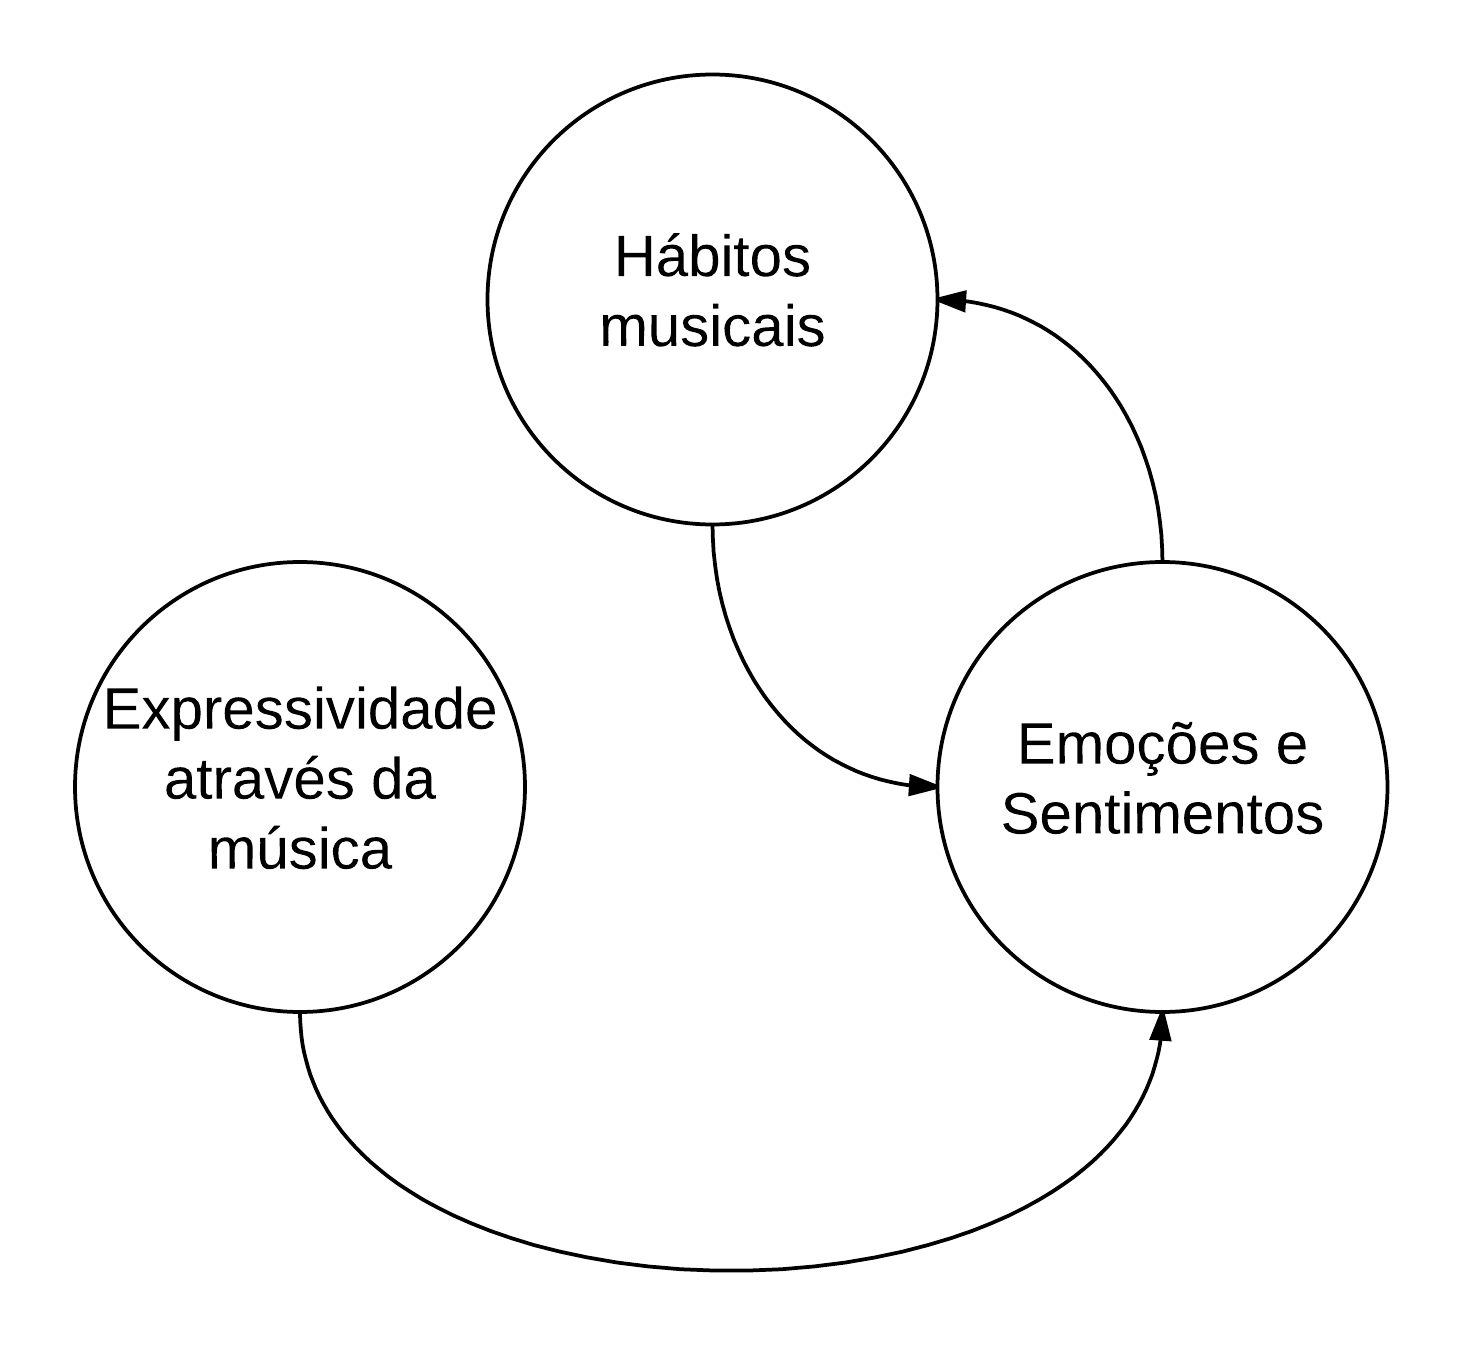
\includegraphics[height=3in, width=3in]{music-mood.png}
\caption{Relação entre expressividade de um artista através de sua música
	e o ciclo criado entre a indução de sentimentos no ouvinte e a escolha
	por músicas que correspondem a seu humor atual.}
\label{fig:music-mood}
\end{figure}

% Música como reflexo das emoções do ouvinte.
% Consumo massivo de música na modernidade - dados/estudo relevantes.
Já sabemos que os hábitos musicais de uma pessoa influenciam diretamente
seu humor, sentimentos e emoções \cite{mccraty1998}. Mais especificamente, existem estudos que demonstram a influência das letras
de uma música no humor e comportamento do ouvinte
\cite{doi:10.2190/35T0-U4DT-N09Q-LQHW}. Esses dois aspectos, aliados
 ao fato de que o consumo de música sofreu grande aumento com a chegada
 das plataformas de streaming digital e compartilhamento de arquivos
 \cite{doi11044343huang} nos fornecem grande indicação
  de que podemos utilizar os hábitos musicais de um ouvinte como fonte de
 informações a respeito do humor e emoções do mesmo.

\section{Problema}

Diante da relação íntima entre humor e hábitos musicais, uma tarefa
particularmente relevante é aquela de identificar usuários (ouvintes)
cujos hábitos de consumo musical denotam possíveis transtornos
psicológicos e de humor. Enquanto esse tipo de análise é muito simplista
para determinar qualquer tipo de transtorno com acurácia, ele pode servir
como um forte indicador de alterações de humor e, como tal, identificador
de usuários que necessitam de algum tipo de suporte emocional.

Plataformas de streaming e recomendação de música online como Last.fm
\cite{haupt2009} e Spotify \cite{5569963}
possuem bases de dados massivas sobre seus usuários
\cite{pichl2014combining} \cite{4736778}, contendo informações
sobre seus artistas favoritos, músicas, álbuns, além de coletar, em tempo
real, informações sobre o hábito musical de um ouvinte. Dessa forma,
essas plataformas a base de dados ideal para a tarefa de identificar 
o humor de um usuário baseado nas músicas que este ouve.

A partir desses dados, é possível coletar os hábitos musicais de um
determinado usuário ao longo de um intervalo de tempo qualquer. Com
esses dados em mão e uma abordagem que envolve tanto os campos de
processamento de linguagem natural - mais especificamente a área
de análise de sentimentos, para tentar posicionar as letras de uma música 
no espectro de emoções humanas -, quanto a área da psicologia e música
em si, podemos tentar extrair, a partir dos hábitos musicais de um
usuário, suas emoções e sentimentos, identificando em último caso aqueles
que demonstram maior necessidade de intervenção e suporte psicológico, 
que pode ser oferecido de várias maneiras diferentes pelas próprias
plataformas.

\section{Modelagem}

% Coleta de dados
O primeiro passo para resolver abordar esse problema é determinar como coletar os dados necessários para traçar um panorama sobre os hábitos
musicais de um usuário. Para isso, a plataforma Last.fm foi escolhida,
não só pela quantidade massiva de dados que acumula, mas também pelo
fato de que todos os seus dados são exibidos publicamente na mesma,
como definido nos termos de contrato do serviço \cite{Lastfmterms}.

% Parâmetros
Nessa etapa é importante definir a quantidade $ n $ para determinar
 as últimas $ n $ músicas que um usuário ouviu. Essa não é uma escolha
 muito simples, uma vez que, para valores muito altos de $ n $, perdemos
 acurácia, no sentido de que essas músicas podem refletir um período de
 tempo muito longo, onde as emoções do usuário podem variado 
 arbitrariamente. Por outro lado, é desejável escolher um valor de $ n $
 suficientemente alto para reunir a maior quantidade possível de músicas
 que refletem um mesmo estado de sentimento/humor do usuário.

% Letras
Em seguida, é preciso reunir os atributos das canções que servirão de 
indicadores para as emoções das mesmas e, consequentemente, dos usuários.
O primeiro atributo a ser considerado são as letras das músicas. Para 
facilitar a implementação do trabalho, só foram levadas em consideração
as músicas cujo idioma é o inglês (uma vez que já existe uma grande
quantidade de ferramentas existentes para trabalhar com esse idioma).

De posse das letras de uma canção, podemos tentar quantificar a negatividade
das palavras. Para isso, podemos usar uma base de dados que já contenha
emoções associadas a cada palavra. Para esse trabalho, foi escolhida
a base \textit{NRC Word-Emotion Association Lexicon}
\cite{Mohammad13}. Além disso, é necessário realizar um pré-processamento
no texto, removendo as flexões das palavras e excluindo aquelas cuja
classe gramatical não seja forte indicador de sentimento ou emoção, i.e.,
palavras como 'hi', 'him', 'there', etc. Com isso, conseguimos quantificar
a porcentagem de palavras negativas nas letras de uma música.

% Músicas instrumentais
Naturalmente, canções instrumentais também devem ser identificadas
e tratadas de forma especial, de modo que também possam ser extraídas 
informações importantes das mesmas.

\section{Implementação}



\section{Estudo de caso}



\section{Conclusão}